

\documentclass{article}
\usepackage[french]{babel}
\usepackage[T1]{fontenc}  % pour french
\usepackage[letterpaper,top=2cm,bottom=2cm,left=3cm,right=3cm,marginparwidth=1.75cm]{geometry}
\usepackage{amsmath}
\usepackage{graphicx}
\usepackage{enumitem}
\usepackage{float}
\usepackage[colorlinks=true, allcolors=blue]{hyperref}

\title{Projet 5 IA: Réseaux de neurones}
\author{Berthion Antoine - 566199}

\begin{document}

\maketitle

\section{Introduction}

\noindent Dans ce rapport, nous analysons l'influence de divers \textbf{paramètres d'entraînement} sur des modèles de \textbf{réseaux de neurones}, et plus particulièrement ceux appartenant à la famille des \textbf{autoencodeurs}. Nous examinons également les \textbf{cas limites} ainsi que le \textbf{phénomène d'hallucination} souvent observé dans ces modèles.

\vspace{-1em}  % plus proche = plus cool (jsp)

\begin{figure}[H]
    \centering
    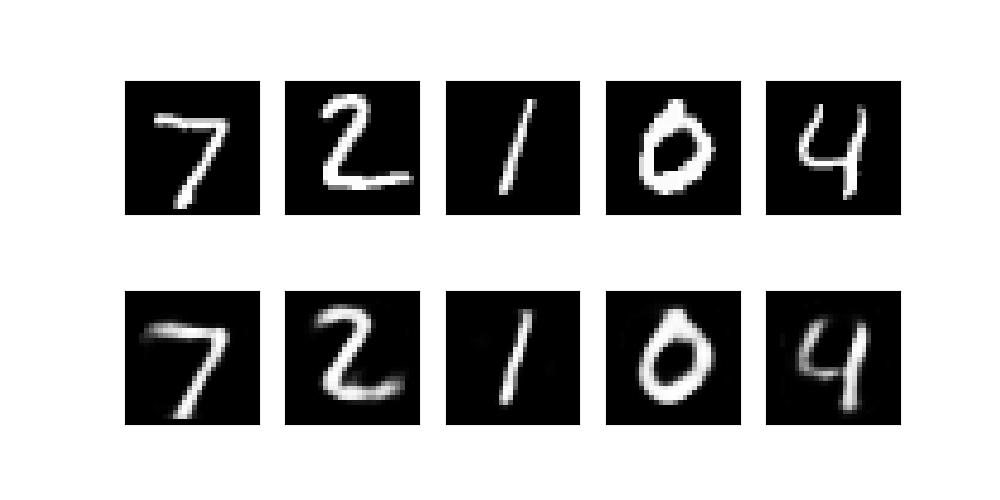
\includegraphics[width=0.7\textwidth]{src/intro.png}
    \caption{Reconstruction des nombres après entraînement du modèle \textbf{mnist}}
    \label{fig:intro}
\end{figure}


\section{Expérimentations}
\label{sec:exp}

\noindent Dans cette section, nous réalisons des expériences sur le paramétrage de l'entraînement de notre modèle. Nous commencerons par décrire le cadre expérimental dans la section \ref{subsec:cadre_exp}, avant de présenter les différents résultats dans la section \ref{subsec:res}. Enfin, la section \ref{sec:disc} sera dédiée à l'analyse de ces résultats.

\subsection{Cadre Expérimental}
\label{subsec:cadre_exp}

\noindent Afin de mener correctement nos expériences, nous ferons varier un seul paramètre à la fois afin d'étudier les effets de ces variations sur les résultats de l'entraînement. Nous mesurerons les résultats, exprimés en termes de pourcentage de perte durant l'encodage et le décodage. Chaque expérience sera répétée cinq fois, et nous calculerons la moyenne des résultats pour assurer leur pertinence. \\

\vspace{-0.5em}

\noindent Nous ferons successivement varier la taille du vecteur compressé $\hat{x}$, la valeur du taux d'apprentissage $\mu$, et enfin le nombre d'époques, noté $e$. Les résultats sont présentés ci-dessous, dans la section \ref{subsec:res}. Dès lors ou les paramètres ne varient pas, les valeurs sont fixées à :

\vspace{0.5em}

\begin{itemize}
    \item Dimension d'encodage de $\hat{x} = 32$
    \item Taux d'apprentissage $\mu = 0.01$
    \item Nombre d'epochs $e = 10$
\end{itemize}


\subsection{Résultats}
\label{subsec:res}

\noindent Dans cette sous-section, nous présenterons de manière succincte les résultats de nos expériences.

\subsubsection{Influence du Learning-Rate}

\vspace{-0.5em}

\begin{figure}[H]
    \centering
    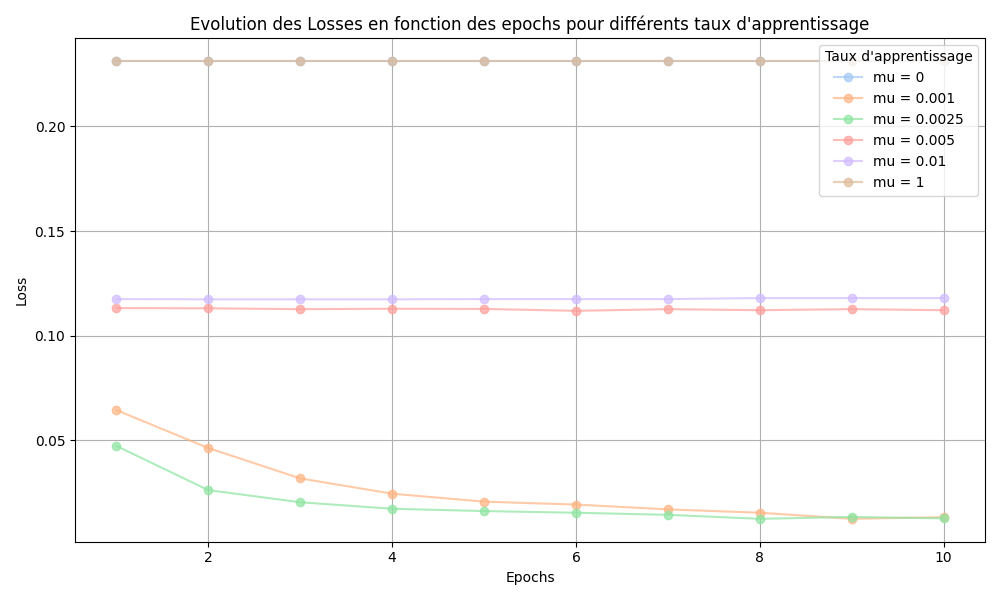
\includegraphics[width=0.9\textwidth]{src/learning_rate.png}
    \vspace{-1em}
    \caption{Influence du \textit{Learning-Rate} $\mu$}
    \label{fig:learning_rate}
\end{figure}

\subsubsection{Influence de la taille du vecteur $\hat{x}$}

\vspace{-1em}

\begin{figure}[H]
    \centering
    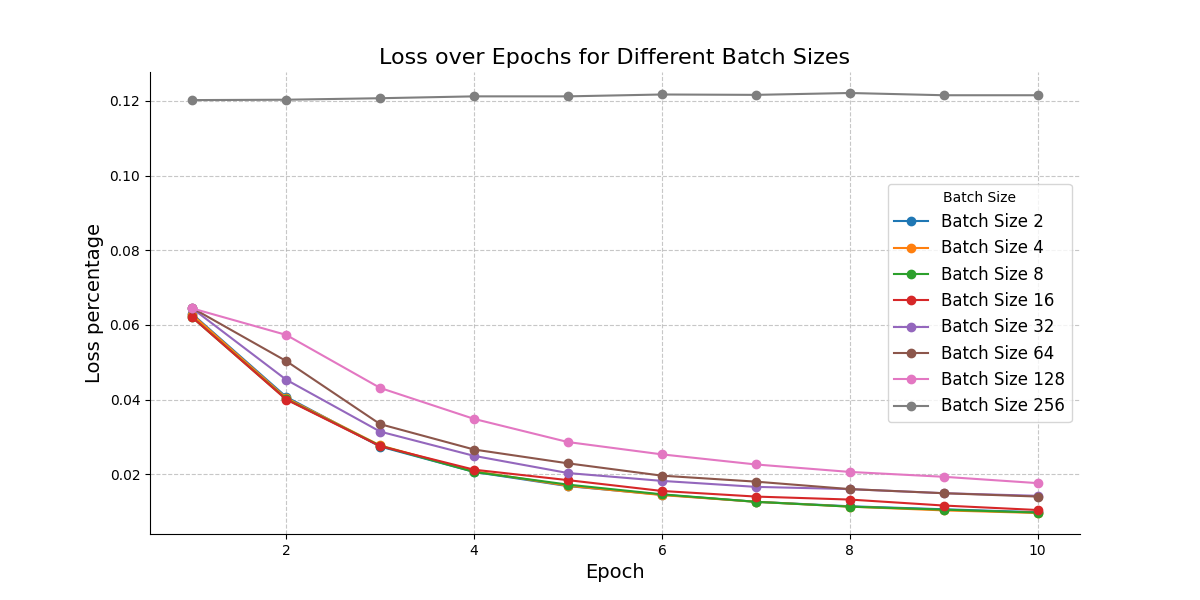
\includegraphics[width=1\textwidth]{src/batchsize.png}
    \vspace{-1em}
    \caption{Influence de la taille du vecteur $\hat{x}$}
    \label{fig:xhat}
\end{figure}

\subsubsection{Influence du nombre d'Epochs}

\vspace{-1em}

\begin{figure}[H]
    \centering
    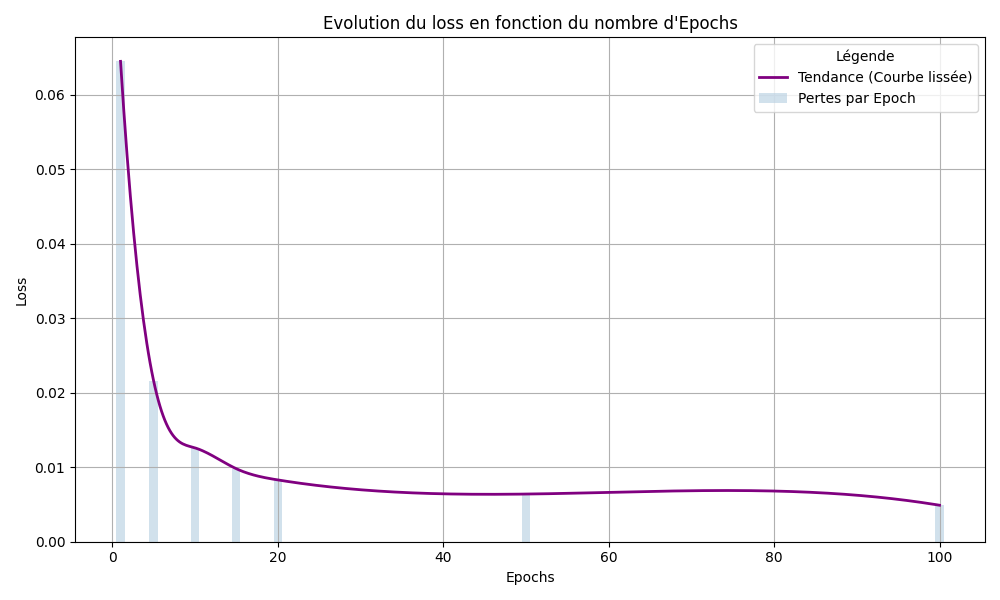
\includegraphics[width=0.9\textwidth]{src/epoch.png}
    \caption{Influence du nombre \textit{d'Epochs} $e$}
    \vspace{-1em}
    \label{fig:epochs}
\end{figure}

\vspace{1em}


\section{Discussion des résultats}
\label{sec:disc}

\noindent Discutons à présent de l'impact de la variation des différents paramètres, testés expérimentalement dans la section \ref{sec:exp}.


\subsection{Variation du learning rate.}
\noindent Nous pouvons observer dans la figure \ref{fig:learning_rate} que les valeurs extrêmes, telles que $0$ et $1$, sont totalement inefficaces. Ces valeurs déterminent la vitesse à laquelle les poids (\textit{weights}) du modèle sont ajustés lors de chaque itération. Une valeur de $0$ empêche toute mise à jour des poids, rendant impossible tout apprentissage. De manière similaire, une valeur de $1$ conduit à des mises à jour trop brutales, empêchant le modèle de converger vers une solution optimale. Les meilleures performances sont observées pour des valeurs comprises entre $0.001$ et $0.003$, ce qui est cohérent avec les bonnes pratiques d'entraînement des réseaux de neurones. En effet, avec un nombre modéré d'\textit{epochs} (autour de $10$), un faible learning rate permet des ajustements progressifs, limitant l'influence des erreurs individuelles. Cette approche évite que le modèle soit fortement perturbé par des fluctuations tardives dans les gradients, dues au bruit dans les données d'entraînement.

\subsection{Variation du nombre d'\textit{epochs}} 
\noindent La figure \ref{fig:epochs} montre que, pour des valeurs faibles, l'augmentation du nombre d'\textit{epochs} améliore significativement la précision du modèle. Cependant, au-delà d'un certain seuil, l'amélioration devient marginale, voire négative, en raison du phénomène de \textit{surapprentissage} (\textit{overfitting}). Ce dernier se produit lorsque le modèle s'adapte trop aux données d'entraînement, perdant ainsi en capacité de généralisation sur des données non vues. Par ailleurs, nous notons que le temps d'entraînement croît de manière linéaire avec le nombre d'\textit{epochs}, ce qui peut rapidement devenir un facteur limitant pour des valeurs élevées. Notre analyse expérimentale suggère qu'un compromis idéal se situe entre $10$ et $20$ \textit{epochs} pour notre problème, offrant un bon équilibre entre précision et temps d'entraînement. Pour les cas extrêmes, une seule \textit{epoch} entraîne des résultats médiocres, tandis qu'une augmentation à seulement deux \textit{epochs} engendre une nette amélioration des performances.

\subsection{Variation de la taille du vecteur encodé $\hat{x}$}
\noindent En guise de dernière partie de cette section, discutons des résultats obtenus dans la figure \ref{fig:xhat}, qui porte sur la taille d'encodage du vecteur $\hat{x}$. Les expériences montrent qu'une taille minimale d'encodage est favorable pour la performance du modèle. Cependant, nous observons que le temps d'entraînement augmente de manière exponentielle à mesure que la taille d'encodage diminue. 

\noindent Plus précisément, les résultats obtenus pour des tailles de vecteur égales à $2$, $4$, et $8$ sont très similaires en termes de perte, mais présentent des différences significatives en termes de temps d'entraînement. Une taille d'encodage de $8$ semble offrir un compromis idéal pour notre modèle, combinant rapidité et performance. Cette taille permet d'obtenir des résultats proches de ceux des vecteurs plus petits, tout en évitant les temps de calcul excessifs associés à des encodages trop compacts.


\section{Phénomène d'hallucination}

\noindent Un aspect intéressant des autoencodeurs est leur comportement face à des vecteurs d'entrée aléatoires, jamais observés durant l'entraînement. Ce phénomène, appelé \textit{hallucination}, correspond à la capacité du modèle à générer des sorties qui ressemblent aux données d'entraînement, bien que l'entrée ne soit pas issue de celles-ci. \\ 

\noindent En soumettant des vecteurs aléatoires, par exemple tirés d'une distribution uniforme ou normale, on observe que l'autoencodeur reconstruit des représentations plausibles dans l'espace des données originales. Cela s'explique par le fait que l'autoencodeur apprend une distribution réduite des données d'entraînement dans l'espace d'encodage. Ainsi, même des vecteurs encodés aléatoires proches de cette distribution génèrent des reconstructions qui reflètent les structures apprises. \\

\noindent Toutefois, si les vecteurs encodés sont trop éloignés de la distribution de l'espace d'encodage, les résultats deviennent incohérents ou chaotiques, mettant en évidence les limites de généralisation du modèle. Ce comportement peut être dangereux dans la mesure ou il pourrait induire les humains en erreur, donnant de très grandes garanties sur des données incohérentes présentant une structure coïncidant par hasard avec une structure apprise pendant l'entraînement du modèle.

\section{Propositions d'améliorations}

\noindent Pour améliorer les performances de l'autoencodeur, nous proposons deux modifications clés au réseau, en nous appuyant sur les principes d'implémentation décrits dans l'énoncé.

\subsection{Ajout de régularisation pour éviter le surapprentissage}

\noindent Le phénomène de surapprentissage (\textit{overfitting}) peut limiter la capacité de généralisation du modèle sur des données non vues. Une approche efficace consiste à ajouter une régularisation $L_2$ (ou poids de décroissance). Cela implique de modifier les mises à jour des poids dans le \textit{backward-forward} en y ajoutant un terme de pénalité proportionnel au carré des poids actuels. La mise à jour des poids pour une couche $W_i$ deviendrait :

\[
W_i = W_i - \mu
\left(
\Delta W_i + \lambda W_i
\right)
\]

\noindent où $\lambda$ est le coefficient de régularisation, et $\Delta W_i$ représente le gradient calculé lors du \textit{backward-forward}. Cette méthode limite les poids extrêmes, favorisant un modèle plus robuste. Une alternative intéressante pourrait être d'utiliser un dropout, qui consiste à désactiver aléatoirement des neurones durant l'entraînement pour éviter la dépendance excessive à certains chemins du réseau.

\subsection{Augmentation de la capacité du modèle avec des couches supplémentaires}

\noindent Une autre amélioration serait d'augmenter la capacité de représentation de l'autoencodeur en ajoutant des couches intermédiaires supplémentaires, aussi bien dans la phase d'encodage que dans celle de décodage. Par exemple, en insérant une nouvelle couche intermédiaire $x_{\text{int}}$ connectée par des matrices de poids $W_{\text{enc}}$ et $W_{\text{dec}}$, les étapes du passage avant (\textit{forward}) deviendraient :

\begin{align*}
x_{\text{enc}} &= \text{activation}(x \cdot W_1) \\
x_{\text{int}} &= \text{activation}(x_{\text{enc}} \cdot W_{\text{enc}}) \\
\hat{x} &= \text{activation}(x_{\text{int}} \cdot W_2) \\
x_{\text{dec\_int}} &= \text{activation}(\hat{x} \cdot W_{\text{dec}}) \\
y &= \text{activation}(x_{\text{dec\_int}} \cdot W_3)
\end{align*}

\noindent Cette approche pourrait permettre au réseau de capturer des structures plus complexes dans les données, à condition de maintenir une régularisation suffisante pour éviter un surapprentissage dû à l’augmentation du nombre de paramètres. \\

\section{Utilisation des LLM}

\noindent Dans cette courte partie, nous discuterons de l'utilisation des LLM dans le cadre du projet. Aucun LLM n'a été utilisé pour l'aspect implémentation ainsi que la compréhension du projet. Cependant, ce rapport à été corrigé du point de vue de la syntaxe et de la grammaire par DeepL ainsi qu'un modèle GPT. Notons tout de même qu'aucune des informations du rapport n'a été produite par une autre personne que l'auteur.

\section{Conclusion}

\noindent Ce rapport a permis d'explorer les performances des autoencodeurs en fonction de divers paramètres d'entraînement, ainsi que d'analyser des phénomènes spécifiques tels que l'hallucination. Nous avons expérimentalement identifié les configurations optimales, notamment pour le learning rate, le nombre d'epochs et la taille du vecteur d'encodage, tout en soulignant les limites imposées par le surapprentissage et la capacité de généralisation. Les propositions d'améliorations, telles que l'ajout de régularisation et l'augmentation de la complexité du réseau, ouvrent des perspectives intéressantes pour renforcer l'efficacité de ces modèles.

\end{document}
